\chapter{Applications of Tensor Structured Coupled Cluster
\label{ch:app_tcc}}

\section{THC-RCCSD method
\label{sec:thc_rccsd}}
\subsection{Introduction}
In this chapter we present the first application of our tensor structured 
coupled cluster theory. We start with the RCCSD method, where both the two body 
interaction part of the Hamiltonian and the ${}^2T$ amplitudes have THC 
structure. Note that ${}^2T$ is never built as a four index tensor, but is 
rather optimized in a decomposed form. This combination of decompositions 
results in a procedure with quartic cost in the basis size $N$ and the ranks of 
THC approximation. Diagrammatically, our choice of decompositions in THC-RCCSD 
can be summarized as:
%
\begin{equation}
\vcenter{\hbox{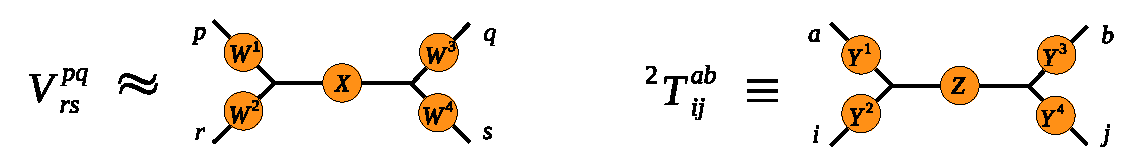
\includegraphics[width=0.9\textwidth]
{figures/thc_rccsd/rccsd_thc_def}}}
.
\label{fig:rccsd_thc_def}
\end{equation}
%
As the diagrams show, the two electron interaction is decomposed in Mulliken 
order, as well as the two body excitation amplitudes. To study the 
properties of THC-RCCSD we calculated energies of a set of small to medium size 
molecules.

\subsection{Computational details}
In our setup the decomposition of the electron interaction tensor was 
calculated with a two step method, as described in 
Ref.~\cite{schutski2017tensor} First, a partial singular value decomposition of 
the integrals in AO basis was calculated. We retained $r_{V}$ singular values 
and vectors. For larger systems, listed in Tab.~\ref{tab:energies_thc_rccsd}, 
RI-decomposed two-electron integrals were used in place of singular 
vectors. Next, a CP decomposition of rank $r_{V}$ of the resulting 
left and right singular vectors (arranged as three index tensors of size $N 
\times N \times r_{V}$) was calculated with ALS. The iterative least squares 
procedure was stopped when the ratio of the objective function $f$ to the 
square of the Frobenius norm of the original tensor dropped below $10^{-14}$, or 
a limit of 1000 iterations was reached.

In the subsequent coupled cluster calculations we chose the rank of the THC 
decomposition of ${}^2T$ amplitudes ($r_{T}$) to be equal to the rank 
used in approximating integrals, e.g. $r_{T} = r_{V}$. 
The CC iterations were stopped either after the energy was converged to within 
$10^{-9}$ Hartree or a limit of 250 iterations 
was reached. All calculations used the cc-pVDZ basis from the EMSL
database,\cite{schuchardt2007basis} and the corresponding cc-pVDZ-RI
was used in the RI approximation. The threshold for pseudoinverses was set to 
$10^{-10}$.

Our code was written in MATLAB and used Gaussian software~\cite{gaussian} 
for the calculation of two-electron integrals and Hartree Fock solutions. We 
also used Tensorlab~\cite{vervliettensorlab} to calculate CPD in the 
decomposition of two-electron integrals.

\subsection{Accuracy of THC for two electron integral approximation}
The accuracy of the THC decomposition of the two-electron integrals governs the
accuracy of the subsequent calculations. Thus, it is important to 
check the dependence of the error in the decomposition of
two-electron integrals on THC rank. Figure~\ref{fig:thc_err_mo_3systems} 
shows this error in a double logarithmic scale for three small molecules. 
Once again, we note that the decomposition is computationally useful if the 
rank $r_\mathrm{V}$ is close to the number of basis functions $N$.  As the 
figure shows, the error in the two-electron integrals decreases exponentially 
with respect to THC rank. We found that this trend holds for every system
tested. Further, there is no significant difference whether the two-electron 
integrals are decomposed in the atomic orbital or molecular orbital basis. As 
is demonstrated in Figure~\ref{fig:thc_err_ao_vs_mo}, the accuracy of the 
decomposition depends only slightly on the choice of the basis, and the ratio 
of errors in different bases is close to one.
%
\begin{figure}[tb]
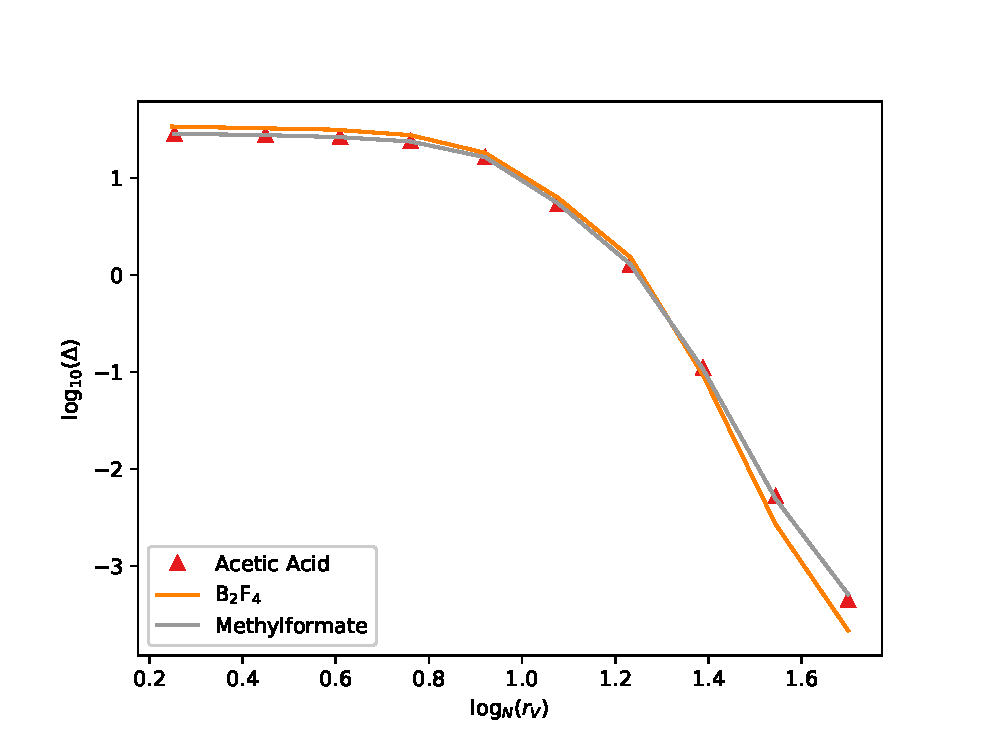
\includegraphics[width=\columnwidth]{figures/thc_rccsd/thc_err_mo_3systems}
\caption{Frobenius norm of error in THC decomposed two-electron integrals, 
atomic orbital basis as the function of rank $r_{V}$
\label{fig:thc_err_mo_3systems}}
\end{figure}
%
\begin{figure}[tb]
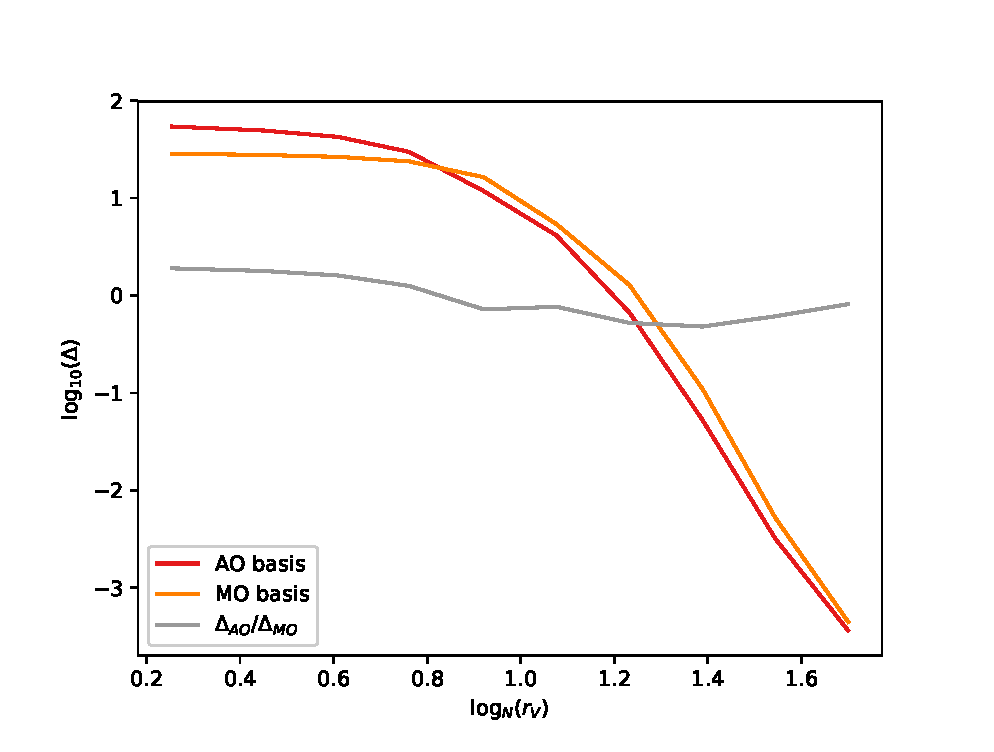
\includegraphics[width=\columnwidth]{figures/thc_rccsd/thc_err_ao_vs_mo}
\caption{Frobenius norm of error in THC decomposed two-electron integrals of 
Acetic Acid in atomic orbital and molecular orbital bases as the function of 
rank $r_{V}$
\label{fig:thc_err_ao_vs_mo}}
\end{figure}
%
To see how the errors in approximation of two-electron 
integrals influence the accuracy of subsequent energies, we checked 
the differences in the second-order M{\o}ller-Plesset (MP2) correlation
energy with respect to the exact MP2 calculation, as shown in 
Fig.~\ref{fig:mp2_err_ao_full}.  The combination
of MP2 and THC was first proposed by Hohenstein \emph{et
al}.\cite{hohenstein_thc2}; the computational effort of the method scales 
as $O(N^4)$.  The way these authors were calculating THC decomposition, however, 
was quite different from ours. As we found, the error in the MP2 correlation 
energy follows the trend seen in the decomposition of the integrals (see 
Fig.~\ref{fig:mp2_err_ao_full}). Results within $0.1~\mathrm{mH}$
of the exact value are already achieved with
$r_\mathrm{V} \sim N^{1.2} - N^{1.4}$.
We expect that the THC would work even better for larger and more extended 
systems as the two-electron integrals become sparser and a lower rank 
decomposition would correspondingly become more accurate.
%
\begin{figure}[tb]
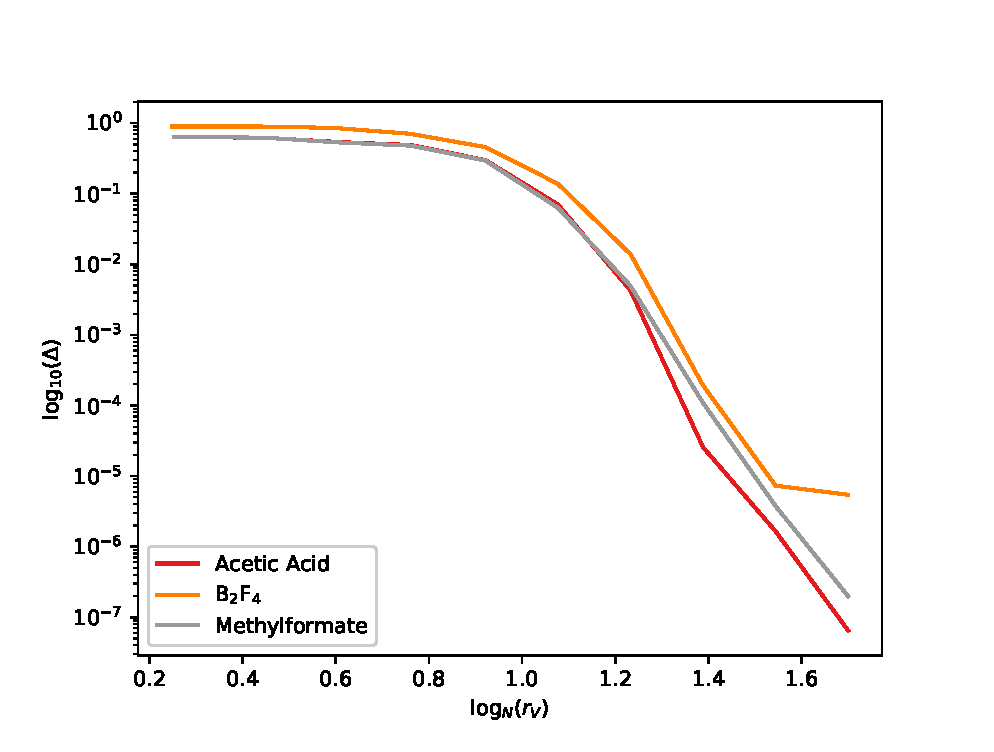
\includegraphics[width=\columnwidth]{figures/thc_rccsd/mp2_err_ao_full}
\caption{Absolute error in the MP2 correlation energy as the function of rank 
$r_{V}$, H
\label{fig:mp2_err_ao_full}}
\end{figure}
%
\subsection{Accuracy of THC-RCCSD}
We are now ready to evaluate the accuracy of the THC-decomposed RCCSD
method. Recall that we set the rank in the decomposition of amplitudes 
equal to the rank used in the decomposition of two electron integrals. The 
error in the RCCSD correlation energy has a non-monotonic dependence on THC 
rank, but follows the 
same basic trends as seen in Fig.~\ref{fig:thc_err_mo_3systems} and
Fig.~\ref{fig:mp2_err_ao_full}. Similarly to the case of MP2, errors on 
the order of $0.1~mH$ are achieved with $r_\mathrm{T} = r_\mathrm{V} \sim 
N^{1.2} - N^{1.4}$.
%
\begin{figure}[tb]
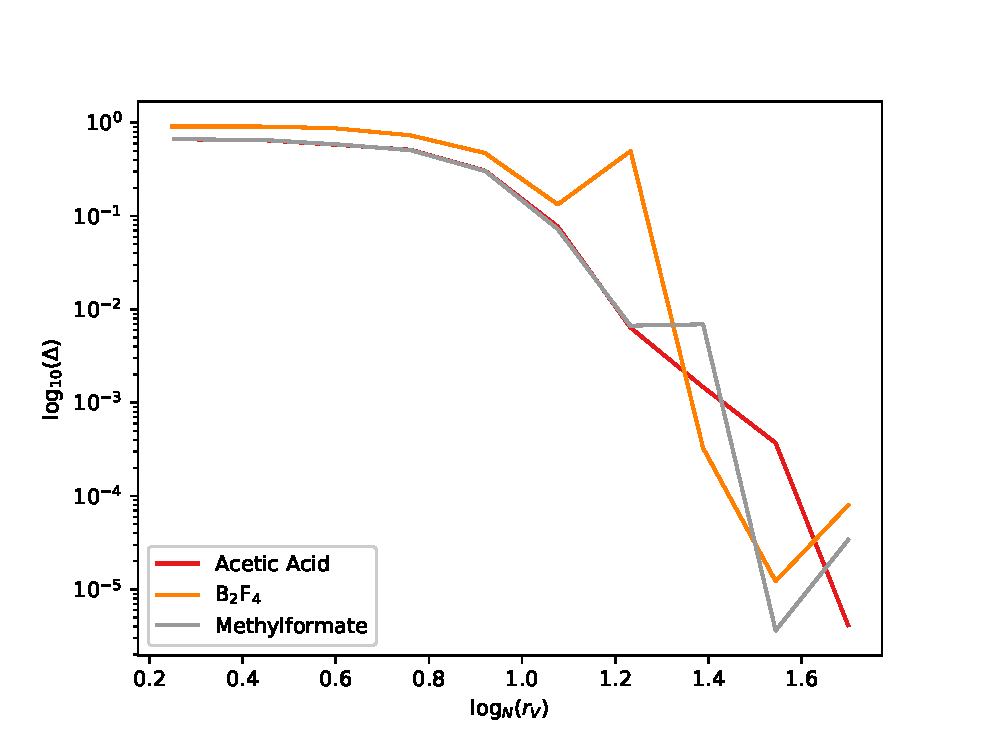
\includegraphics[width=\columnwidth]{figures/thc_rccsd/cc_err_ao_full}
\caption{Absolute error in the RCCSD correlation energy as the function of 
ranks of THC decomposed ${}^2T$ amplitudes and two-electron integrals 
$r_{T} = r_{V}$, H
\label{fig:cc_err_ao_full}}
\end{figure}
%
It is interesting to estimate what part of the error in energy can be
attributed to the approximation of the Hamiltonian only. For this reason we 
calculated the correlation energy with converged THC-RCCSD amplitudes but exact
two-electron integrals.  As Fig.~\ref{fig:cc_err_ao_full_amps_only}
shows, using the exact two-electron integrals substantially decreases the error 
in energy, which later motivated us to look for better ways of decomposing the 
two-electron integrals. The non-monotonic behavior of the error (as compared to 
MP2) can be attributed to the nonlinear nature of the coupled cluster 
equations, which can be quite sensitive to changes in the parameters of the 
Hamiltonian.
%
\begin{figure}[tb]
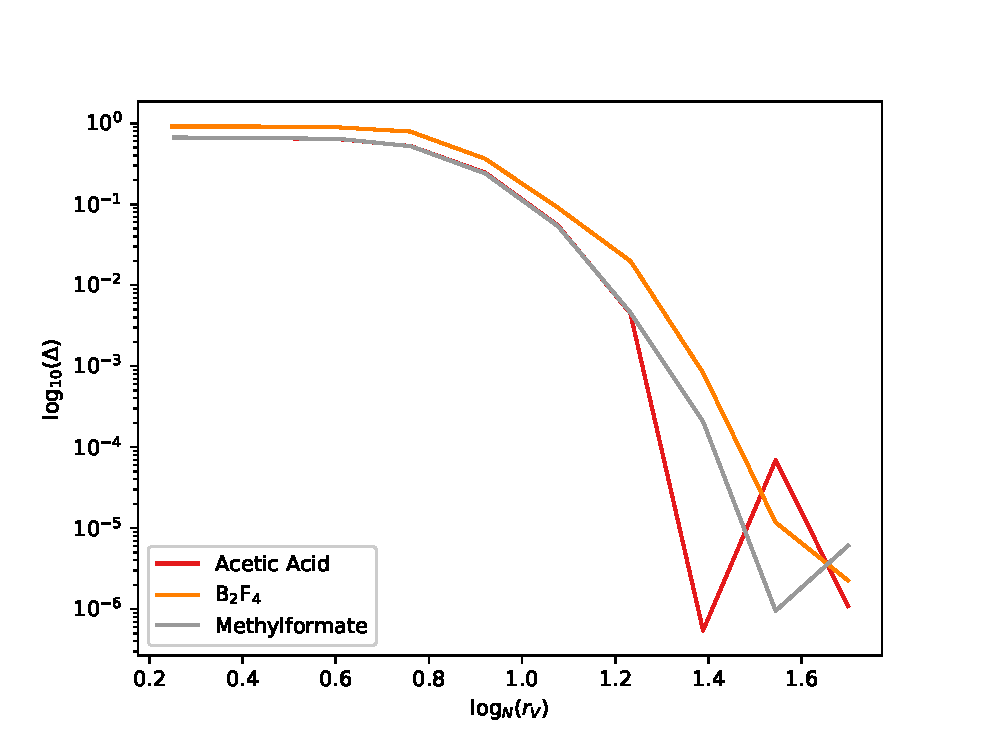
\includegraphics[width=\columnwidth]{figures/thc_rccsd/cc_err_ao_full_amps_only}
\caption{Absolute error in the RCCSD correlation energy with exact two-electron 
integrals and THC decomposed ${}^2T$ amplitudes as a function of rank $r_{T}$, H
\label{fig:cc_err_ao_full_amps_only}}
\end{figure}
%
\subsection{Convergence of THC-RCCSD}
As the solution of THC-RCCSD is found iteratively, an important question is 
the convergence of this method. We used a simple iterative algorithm to 
solve THC-RCCSD equations, and stopped updates when a specified difference in 
energy between subsequent steps was reached. The convergence of the resulting 
method significantly depends on the rank of the THC approximation. 
Figure~\ref{fig:cc_thc_convergence} shows the number of iterations the 
algorithm had to take to reach $10^{6} ~ \mathrm{H}$ difference 
in energy between steps.
%
\begin{figure}[tb]
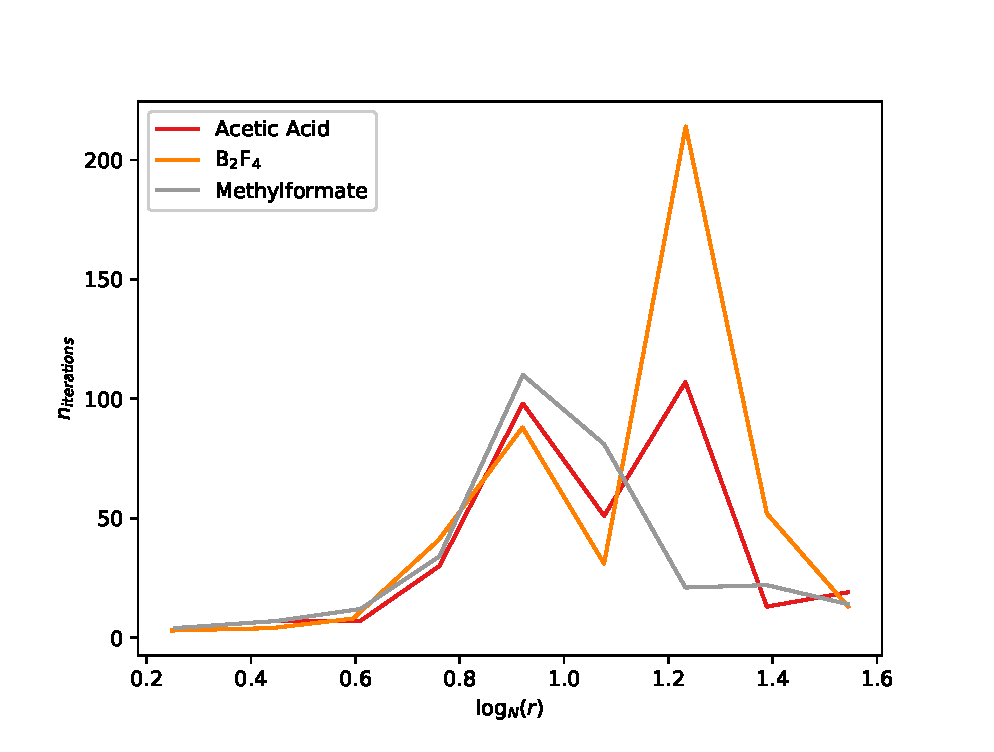
\includegraphics[width=\columnwidth]{figures/thc_rccsd/niter_vs_logr}
\caption{Number of iterations of THC-RCCSD to reach $1 \cdot 10^{-6} H$ 
difference in energy between updates}
\label{fig:cc_thc_convergence}
\end{figure}
%
For small as well as larger THC ranks the convergence of THC-RCCSD is 
comparable or better than regular RCCSD (if solved by simple iteration). 
In the intermediate regime, however, the algorithm may need
a large number of iterations or fails to converge. We note that the 
convergence in this regime significantly depends on the choice of initial 
parameters. This behavior can possibly be explained by the fact that THC-RCCSD 
in our formulation is a sum of two iterative algorithms, namely, an ALS step 
and 
a CC iteration. These two parts of THC-RCCSD can generate competing updates, 
depending on the magnitude of the rank. In case of small ranks the update 
should be mostly determined by ALS, as ${}^{2}T$ amplitudes are poorly 
approximated with any set of parameters $Y$. In contrast, with larger ranks 
mostly the CC step dominates the update, because ${}^2T$ is well 
approximated at each step. We admit, however, that the means to control 
convergence of our hybrid algorithms may need further study. All of the 
calculations in Table~\ref{tab:energies_thc_rccsd} were done in a regime where 
THC-RCCSD performs similarly to regular RCCSD, e. g. where THC ranks are 
relatively large. 

\subsection{{THC-RCCSD for weakly correlated systems}
\label{sec:thc_weakly_correlated}}
Having checked the properties of THC-RCCSD on a few small systems, we 
tested the method on a larger set of small and medium-sized molecules introduced 
in previous work on THC.\cite{hohenstein_thc3} Technical details of the 
calculations, including molecular geometries and reference energies, are 
provided in the supplementary materials of Ref.~\cite{schutski2017tensor}. We 
chose the ranks of the THC decomposition of the amplitudes and integrals to be 
on the same scale as the number of auxiliary basis functions $N_\mathrm{RI}$ 
used in the standard RI approximation. In Table~\ref{tab:energies_thc_rccsd} we 
list 
energies, differences with respect to regular Coupled Cluster and the norm of 
final residuals. We used RI for all these calculations 
in the first step of THC decomposition of the two electron integrals. 
%
\begin{center}
\begin{table}[!ht]
\caption{CCSD correlation energies ($E_c$), errors in
correlation energies ($\Delta E_c$) 
and the norm of doubles residuals ($|{}^2R_{ij}^{ab}|$) for several small 
molecules.
\label{tab:energies_thc_rccsd}}
\begin{tabular}{lccccc}
\hline \hline
& & \multicolumn{2}{c}{$\Delta E_c (mH)$} & 
\multicolumn{2}{c}{$|{}^2R_{ij}^{ab}|$}\\
\cline{3-4} \cline{5-6} System & $E_c (mH)$ & $N_\mathrm{RI}$ &
$1.5 \, N_\mathrm{RI}$ & $N_\mathrm{RI}$ &
$1.5 \, N_\mathrm{RI}$\\
\hline
Acetic acid & -666.510 & -0.579 & -0.453 & 0.041 & 0.033 \\
Aniline & -997.193 & -1.177 & -0.471 & 0.051 & 0.032 \\
Diboron tetrafluoride & -909.944 & -0.702 & -0.716 & 0.053 & 0.034\\
Benzene & -823.101 & -0.985 & -0.450 & 0.048 & 0.030\\
Butadiene & -581.340 & -0.710 & -0.274 & 0.041 & 0.025\\
Cyclobutane & -621.099 & -0.895 & -0.290 & 0.039 & 0.028\\
Dimethylsulfoxide & -661.870 & 0.195 & -0.624 & 0.056 & 0.025\\
Furan & -736.463 & -0.865 & -0.454 & 0.046 & 0.033\\
Isobutane & -652.505 & -0.876 & -0.263 & 0.035 & 0.025\\
Methylformate & -666.805 & -0.586 & -0.455 & 0.042 & 0.032\\
Methylnitrite & -708.990 & -0.476 & -0.492 & 0.047 & 0.033\\
Phenol & -1005.727 & -0.887 & -0.514 & 0.051 & 0.032\\
Pyridine & -842.453 & -1.045 & -0.475 & 0.047 & 0.032\\
Pyrrole & -727.051 & -0.855 & -0.407 & 0.045 & 0.032\\
Thiophene & -695.593 & -1.013 & -0.657 & 0.039 & 0.032\\
Toluene & -980.030 & -1.270 & -0.461 & 0.063 & 0.042\\
\hline
mean unsigned error & & 0.820 & 0.466 & &\\
maximum unsigned error & & 1.270 & 0.716 & &\\
root-mean-square error & & 0.861 & 0.482 & &\\
\hline\hline
\end{tabular}
\end{table}
\end{center}
%
As the table shows, already with moderate ranks on the order of the basis size 
excellent accuracy is attained (differences are below $1 ~ \mathrm{mH}$). The 
error of the approximation decreases as we increase the rank. Let us 
also point to an important finding in Table~\ref{tab:energies_thc_rccsd}. As 
THC-RCCSD is an approximation to regular CC equations, the full residuals may 
not be zero, because the number of CC equations is usually much larger than the 
number of parameters of THC-RCCSD. An interesting observation is that while 
the norm of the double residuals is not negligible in THC-RCCSD, the errors in 
energy are quite low. This contrasts with conventional CC, where the 
difference of energy during iterations with the converged value  
is of the same order as the norm of the residual. This fact is explored in 
more detail in the next chapter. 

\subsection{Conclusions}
The development of the THC-RCCSD method is our first application of the tensor 
structured coupled cluster approach.\cite{schutski2017tensor} THC-RCCSD provides 
a viable approximation to conventional RCCSD and should be orders of magnitude 
faster per iteration, especially for large basis sizes $N$. 

It should be noted, however, that most of the time in our 
calculations was spent on the decomposition of the Hamiltonian rather
than on the solution of approximated CC equations. 
One way to overcome this problem is to use quadrature based methods for 
building THC of the electron interaction tensor, such as the ones developed by 
the group of Martinez.\cite{hohenstein_thc1},\cite{parrish2013discrete} These 
methods may be much faster than iterative approaches we employed, at the 
expense of using about 3x larger ranks to reach the same 
accuracy.\cite{parrish2013discrete} Another way is to avoid THC decomposition 
of two electron integrals altogether, as we will do in the next
section.

An important aspect not covered in our work on THC-RCCSD here is its behavior 
in the strong correlation regime. As was mentioned earlier, conventional 
restricted 
CC methods fail at strong correlation. We will return to the 
discussion of the strong correlation regime in 
Chapter~\ref{sec:strong_correlation}